\begin{frame}
	\frametitle{Kalman Filter}
	\note{información extraida de https://youtu.be/PiCC-SxWlH8}
	
	\begin{itemize}
		\item Es un Filtro de Bayes
		\item Todo es Gaussiano
		\begin{equation*}
			p(x)=\det(2\pi\covariance)^{\dfrac{1}{2}} \exp\left(-\dfrac{1}{2} (x - \mu )^{\top} \inverse{\covariance} (x - \mu )  \right)
		\end{equation*}
		
		\item Soluciones optimas para modelos lineales y distribuciones Gaussianas.
	\end{itemize}

	\begin{figure}[!h]
		\centering
		\subfloat[]
		{
			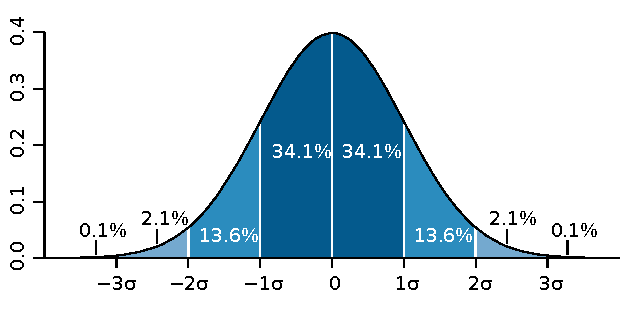
\includegraphics[width=0.3\columnwidth]{./images/standard_deviation_diagram.pdf}
		}
		\subfloat[AGREGAR ELIPSE ELIPSOIDE ]
		{
			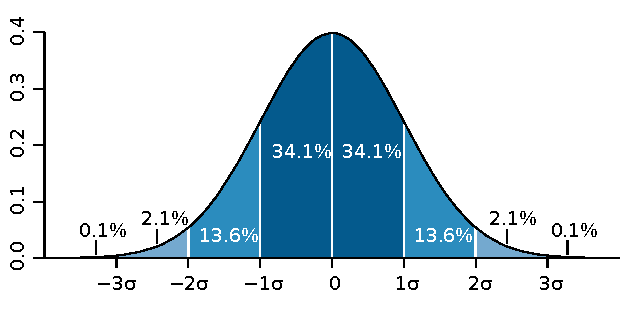
\includegraphics[width=0.3\columnwidth]{./images/standard_deviation_diagram.pdf}
		}
	\end{figure}
\end{frame}


\begin{frame}
	\frametitle{Kalman Filter Asumciones}
	\note{información extraida de https://youtu.be/PiCC-SxWlH8}
	
	
\end{frame}

\begin{frame}
	\frametitle{Sistemas dinámicos no Non-lineales}
	\note{información extraida de https://youtu.be/PiCC-SxWlH8}
	
	
\end{frame}

\begin{frame}
	\frametitle{Motion model linearizado}
	\note{información extraida de https://youtu.be/PiCC-SxWlH8}
	
	
\end{frame}

\begin{frame}
	\frametitle{Observation model linearizado}
	\note{información extraida de https://youtu.be/PiCC-SxWlH8}
	
	
\end{frame}

\begin{frame}
	\frametitle{Algoritmo de Filtro de Kalman Extendido}
	\note{información extraida de https://youtu.be/PiCC-SxWlH8}
	
	
\end{frame}


\begin{frame}
	\frametitle{EKF Localización for feature-based map}
	\note{información extraida de https://youtu.be/PiCC-SxWlH8}
	
	
\end{frame}

\begin{frame}
	\frametitle{Odometry as controls}
	\note{información extraida de https://youtu.be/PiCC-SxWlH8}
	
	
\end{frame}

\begin{frame}
	\frametitle{Motion model}
	\note{información extraida de https://youtu.be/PiCC-SxWlH8}
	
	
\end{frame}

\begin{frame}
	\frametitle{Jacobianos del motion model}
	\note{información extraida de https://youtu.be/PiCC-SxWlH8}
	
	
\end{frame}

\begin{frame}
	\frametitle{Observation model}
	\note{información extraida de https://youtu.be/PiCC-SxWlH8}
	
	
\end{frame}

\begin{frame}
	\frametitle{Jacobianos del observation model}
	\note{información extraida de https://youtu.be/PiCC-SxWlH8}
	
	
\end{frame}

\begin{frame}
	\frametitle{Algoritmo de Filtro de Kalman Extendido}
	\note{información extraida de https://youtu.be/PiCC-SxWlH8}
	
	
\end{frame}

\begin{frame}
	\frametitle{Algoritmo de Filtro de Kalman Extendido}
	\note{información extraida de https://youtu.be/PiCC-SxWlH8}
	
	
\end{frame}

\begin{frame}
	\frametitle{Prediction step}
	\note{información extraida de https://youtu.be/PiCC-SxWlH8}
	
	
\end{frame}

\begin{frame}
	\frametitle{Algoritmo de Filtro de Kalman Extendido}
	\note{información extraida de https://youtu.be/PiCC-SxWlH8}
	
	
\end{frame}

\begin{frame}
	\frametitle{Medición esperada}
	\note{información extraida de https://youtu.be/PiCC-SxWlH8}
	
\end{frame}

\begin{frame}
	\frametitle{Correction step}
	\note{información extraida de https://youtu.be/PiCC-SxWlH8}
	
\end{frame}

\begin{frame}
	\frametitle{2D EKF Localization Ejemplo}
	\note{información extraida de https://youtu.be/PiCC-SxWlH8}
	
\end{frame}

\begin{frame}
	\frametitle{EKF resumen}
	\note{información extraida de https://youtu.be/PiCC-SxWlH8}
	
\end{frame}

